\documentclass{beamer}
\usetheme{metropolis}
\setbeamercolor{background canvas}{bg=white}
\usepackage{graphicx}
\graphicspath{{../dissertation/graphics/}}
\usepackage{natbib}
\usepackage{lmodern}
\usepackage[most]{tcolorbox}
\usepackage{tabularx}
\usepackage{colortbl} 
\newcolumntype{Y}{>{\centering\arraybackslash}X}
\newtcolorbox[blend into=tables]{colortable}[2][]{
	colback=white,
	tabularx*={\renewcommand{\arraystretch}{1.0}}{Y|Y|Y|Y|Y|Y},title={#2},boxrule=0.8pt, center title
}

\title{Hyper Heuristic Cryptography with Mixed Adversarial Nets}
\date{\today}
\author{\textbf{Author:} Aly Shmahell \\ \textbf{Supervisor:} Prof. Giovanni De Gasperis}
\institute{University of L'Aquila}
\begin{document}
	\maketitle
	\section{Introduction}
		\begin{frame}{Q.: What is this dissertation about? A.: Neural Cryptography}
			\textbf{Neural Cryptography:} is an interdisciplinary field in Computer Science, combining both artificial intelligence and cryptography, towards the development of stochastic methods,
			based on artificial neural networks, for use in encryption and cryptanalysis.\\
			\textbf{Hyper Heuristic Cryptography with Mixed Adversarial Nets} adds to the latest experiments in neural cryptography, building upon methodologies presented in a new paper released in 2016 by Google Brain.~\citep{DBLP:journals/corr/AbadiA16}\\
			These methodologies utilize Adversarial Convolutional Neural Networks.
		\end{frame}
		\begin{frame}{Current State of Neural Cryptography}
			\scriptsize{\begin{itemize}
				\item \textbf{Neural Cryptography is viable:} The introduction of convolutional networks provides a well tested and understood methodology in reducing problems where local spatial relations in the data matter, which is the case for cryptography.
				\item \textbf{Neural Cryptanalysis is viable:} Having a mixed convolutional net with fully connected layers will teach the network to account for global spatial relations as well, which teaches the net to learn and counter cryptanalysis.
				\item \textbf{Neural Cryptography can be fast:} A result of using convolutions is that the small-sized pattern-finding filter has shared weights (and biases) for all spatial locations which the convolution processes, and this reduces the compute-power required for the whole process compared to other network models.
				\item \textbf{Neural Cryptography is evolved opposite to being patched:} Adversarial computation has been proven to be effective for years in the form of Genetic Algorithms, and adding adversary as a non-supervised generative model provides a better and easier experiment on how to synthesize a new form of cryptography.
			\end{itemize}}
		\end{frame}
	\section{Neural Mechanisms for Synthesizing Cryptography}
		\begin{frame}{Dummy Net Example}
			\begin{center}
				\includegraphics[width=0.9\textwidth]{SimpleNetDiagram}
			\end{center}
		\end{frame}
		\begin{frame}{1D Convolution}
			\textbf{1D Convolution:} is the process of using a small window (a filter) to determine local spatial relations over a 1D data sample, regardless of whether the sample is inside an n-D data batch.\\
			\textbf{In practice,} it is an algorithmic utilization of matrix multiplications between the filter and consecutive spatial locations in the sample.\\
			\scriptsize{\begin{itemize}
				\item When 1D Convolution is performed on a batch of samples, the batch should be expanded to 3D (by injecting a z-axis within the y-axis).
				\item When convoluting over 3D data, the filter should be 3D as well. 
			\end{itemize}}
		\end{frame}
		\begin{frame}{1D Convolution - Continued}
			\begin{center}
				\includegraphics[height=0.9\textheight]{numpy-3Dtensor-axis}
			\end{center}
		\end{frame}
		\begin{frame}{Simple ConvNet Example with 2 Conv Layers}
			\begin{center}
				\includegraphics[height=0.9\textheight]{convLayerExample}
			\end{center}
		\end{frame}
		\begin{frame}{Simple ConvNet Example with 2 Conv Layers - Continued}
				\begin{center}
					\includegraphics[height=0.2\textheight]{input1}
				\end{center}
				\begin{center}
					\includegraphics[height=0.2\textheight]{input2}
				\end{center}
				\begin{center}
						\includegraphics[height=0.2\textheight]{input3}
				\end{center}
		\end{frame}
		\begin{frame}{Simple ConvNet Example with 2 Conv Layers - Continued}
			\begin{center}
				\includegraphics[height=0.35\textheight]{input_final}\hfill
				\includegraphics[height=0.35\textheight]{input_reshaped}
			\end{center}
			\begin{center}
				\includegraphics[height=0.3\textheight]{filter1}
			\end{center}
		\end{frame}
		\begin{frame}{Simple ConvNet Example with 2 Conv Layers - Continued}
			\begin{center}
				\includegraphics[height=0.8\textheight]{firstConvSample_step2}
			\end{center}
		\end{frame}
		\begin{frame}{Simple ConvNet Example with 2 Conv Layers - Continued}
			\begin{center}
				\includegraphics[height=0.8\textheight]{firstConvSample_step3}
			\end{center}
		\end{frame}
		\begin{frame}{Simple ConvNet Example with 2 Conv Layers - Continued}
			\begin{center}
				\includegraphics[height=0.6\textheight]{firstConvSample_final}
			\end{center}
		\end{frame}
		\begin{frame}{Simple ConvNet Example with 2 Conv Layers - Continued}
			\begin{center}
				\includegraphics[height=0.4\textheight]{secondinput_final}
			\end{center}
			\begin{center}
				\includegraphics[height=0.4\textheight]{filter2}
			\end{center}
		\end{frame}
		\begin{frame}{Simple ConvNet Example with 2 Conv Layers - Continued}
			\begin{center}
				\includegraphics[height=0.9\textheight]{secondConvSample_step1}
			\end{center}
		\end{frame}
		\begin{frame}{Simple ConvNet Example with 2 Conv Layers - Continued}
			\begin{center}
				\includegraphics[height=0.9\textheight]{secondConvSample_step2}
			\end{center}
		\end{frame}
		\begin{frame}{Simple ConvNet Example with 2 Conv Layers - Continued}
			\begin{center}
				\includegraphics[height=0.5\textheight]{secondConvSample_final}
			\end{center}
		\end{frame}
		\begin{frame}{Simple ConvNet Example with 2 Conv Layers - Continued}
			\begin{center}
				\includegraphics[height=0.8\textheight]{squeeze}
			\end{center}
		\end{frame}
		\begin{frame}{Activation Functions after each Layer}
			\begin{itemize}
				\item $" Sigmoid \rightarrow LeakyRealu \rightarrow Sigmoid "$.
				\item $" Tanh \rightarrow LeakyRealu \rightarrow Tanh "$.
				\item $" Sigmoid \rightarrow LeakyRealu \rightarrow Tanh "$.
			\end{itemize}
			The choice was made to use: $" Sigmoid \rightarrow LeakyRealu \rightarrow Tanh "$.
		\end{frame}
		\begin{frame}{Activation Functions after each Layer - Numerical Analysis}
			$" Tanh \rightarrow LeakyRealu \rightarrow Tanh "$.
			\begin{center}
				\includegraphics[height=0.9\textheight]{tanh_leakyRelu_tanh}
			\end{center}
		\end{frame}
		\begin{frame}{Activation Functions after each Layer - Numerical Analysis}
			$" Sigmoid \rightarrow LeakyRealu \rightarrow Sigmoid "$.
			\begin{center}
				\includegraphics[height=0.9\textheight]{sigmoid_leakyRelu_sigmoid}
			\end{center}
		\end{frame}
		\begin{frame}{Activation Functions after each Layer - Numerical Analysis}
			$" Sigmoid \rightarrow LeakyRealu \rightarrow Tanh "$.
			\begin{center}
				\includegraphics[height=0.9\textheight]{sigmoid_leakyRelu_tanh}
			\end{center}
		\end{frame}
		\section{Scheme Structures}
		\begin{frame}{Symmetric Scheme}
			\begin{center}
				\includegraphics[height=0.9\textheight]{symmetricScheme}
			\end{center}
		\end{frame}
		\begin{frame}{Asymmetric Scheme}
			\begin{center}
				\includegraphics[height=0.9\textheight]{asymmetricScheme}
			\end{center}
		\end{frame}
		\begin{frame}{Transfer Learning}
			\textbf{Transfer Learning:} Given a source domain $ D_{S} $
			and learning task $ T_{S} $ , a target domain $ D_{T} $ and learning task
			$ T_{T} $ , transfer learning aims to help improve the learning of the
			target predictive function $ f_{T}(\cdot) $ in $ D_{T} $ using the knowledge in
			$ D_{S} $ and $ T_{S} $ , where $ D_{S} \neq D_{T} $ , or $ T_{S} \neq T_{T} $.~\citep{5288526}
		\end{frame}
		\begin{frame}{Hybrid Scheme}
			\begin{center}
				\includegraphics[height=0.9\textheight]{hybridScheme}
			\end{center}
		\end{frame}
		\section{Project Structure}
		\begin{frame}{Class Diagram}
			\begin{center}
				\includegraphics[height=0.9\textheight]{classDiagram}
			\end{center}
		\end{frame}
		\section{Results}
		\begin{frame}{Thesis Results - Symmetric Training}
			\begin{center}
				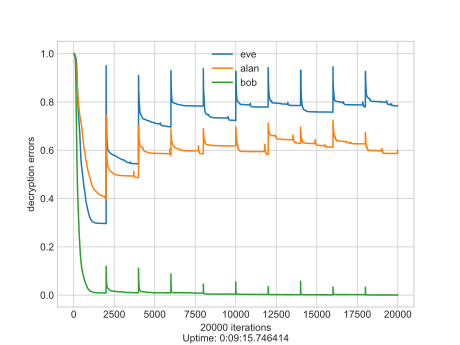
\includegraphics[height=0.9\textheight]{neurencoder-symmetric-training}
			\end{center}
		\end{frame}
		\begin{frame}{Thesis Results - Symmetric Testing}
			\begin{center}
				\includegraphics[height=0.9\textheight]{neurencoder-symmetric-testing}
			\end{center}
		\end{frame}
		\begin{frame}{Thesis Results - Asymmetric Training}
			\begin{center}
				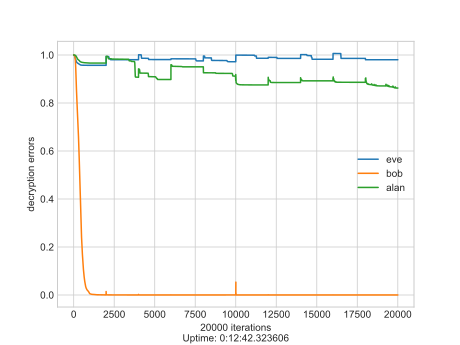
\includegraphics[height=0.9\textheight]{neurencoder-asymmetric-training}
			\end{center}
		\end{frame}
		\begin{frame}{Thesis Results - Asymmetric Testing}
			\begin{center}
				\includegraphics[height=0.9\textheight]{neurencoder-asymmetric-testing}
			\end{center}
		\end{frame}
		\begin{frame}{Thesis Results - Hybrid Training}
			\begin{center}
				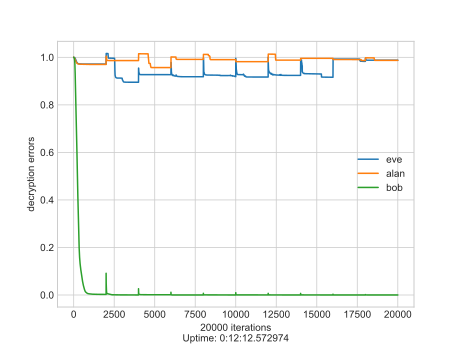
\includegraphics[height=0.9\textheight]{neurencoder-hybrid-training}
			\end{center}
		\end{frame}
		\begin{frame}{Thesis Results - Hybrid Testing}
			\begin{center}
				\includegraphics[height=0.9\textheight]{neurencoder-hybrid-testing}
			\end{center}
		\end{frame}
		\begin{frame}{Symmetric Results from Google Brain - for Comparison}
			\begin{center}
				\includegraphics[height=0.8\textheight]{cryptolearn_batch_tighter}
			\end{center}
		\end{frame}
		\begin{frame}{Asymmetric Results from Google Brain - for Comparison}
			\begin{center}
				\includegraphics[height=0.8\textheight]{pubkey_bob_v_eve}
			\end{center}
		\end{frame}
		\begin{frame}
			\frametitle{References}
			\bibliographystyle{unsrt}
			\bibliography{../dissertation/latex_files/neurencoder.bib}
		\end{frame}
\end{document}
